\documentclass[a4paper]{article}
\usepackage[utf8]{inputenc}
\usepackage[a4paper, left=2.5cm, right=2.5cm, top=2cm, bottom=2cm]{geometry}
\usepackage{lmodern}
\usepackage[T1]{fontenc}
\usepackage{graphicx}
\usepackage{amssymb}
\usepackage[utf8]{inputenc}
\usepackage{pgfplots}
\pgfplotsset{width=6cm,compat=1.9}
\usepackage{multicol}
\usepackage{csquotes}

\renewcommand{\thesection}{\Alph{section}}
\renewcommand{\thesubsection}{\arabic{subsection}}
\renewcommand{\thesubsubsection}{(\emph{\alph{subsubsection}})}

\title{Exponentielle}
\author{Hugo Lageneste}
\date{Janvier 2020}

\begin{document}

{Mathématiques - Exponentielle}

\begin{center}
 \newcommand{\HRule}{\rule{\linewidth}{0.5mm}}
 {\huge \bfseries Exponenteille}\\[0.1cm]
\end{center}

\section{Propriétés de l'exponentielle}
\subsection{Caractérisation}

{La fonction exponentielle notée $\exp{}$ et définie sur $I=\mathbb{R}$ est définie par $\exp{x}=e^x$}

\begin{multicols}{3}
	\begin{itemize}
  		\item{$\exp{}$ est dérivable sur $\mathbb{R}$}
  		\item{$\exp{}\prime x=\exp{x}$}
  		\item{$\exp{0}=1$}
	\end{itemize}
\end{multicols}

\subsection{Propriété}

\[\exp{x+y}=\exp{x} \times \exp{y}\]

\subsection{Signe}

{$\forall x \in \mathbb{R}$, $e^x > 0$}

\begin{center}
	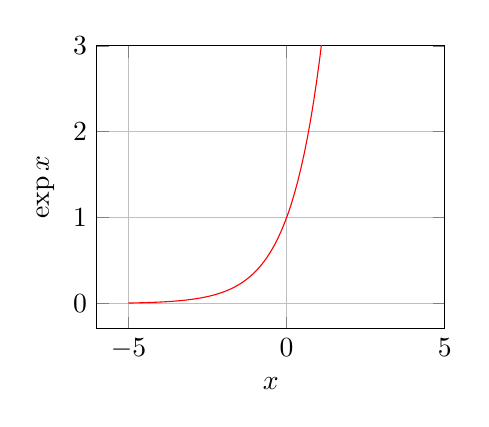
\begin{tikzpicture}
		\begin{axis}[grid=major,  xmax=5, ymax=3, samples=100, xlabel=$x$, ylabel=$\exp{x}$]
			\addplot[color=red]{exp(x)};
		\end{axis}
	\end{tikzpicture}
\end{center}

\subsection{Propriétés algébriques}

{Soient $\forall x, y \in \mathbb{R}$}

\begin{multicols}{2}
	\begin{itemize}
  		\item{$e^x = e^y \Leftrightarrow x=y$}
  		\item{$e^x < e^y \Leftrightarrow x < y$}
	\end{itemize}
\end{multicols}
{$\forall x \in \mathbb{R}^{+*}$ et $\forall n \in \mathbb{Z}$:}

{La fonction exponentielle vérifie les règles des puissances}
{$\forall x,y \in \mathbb{R}$ et $\forall n \in \mathbb{Z}$}

\begin{multicols}{4}
	\begin{itemize}
		\item{$e^{x+y}=e^x e^y$}
		\item{$e^{-x}=\frac{1}{e^x}$}
		\item{$e^{x-y}=\frac{e^x}{e^y}$}
		\item{$(e^{x})^n=e^{nx}$}
	\end{itemize}
\end{multicols}

\section{Étude de l'exponentielle}
\subsection{Limites}

{Aux bornes de son ensemble de définition, les limites de l'exponentielle sont:}

\begin{multicols}{2}
	\begin{itemize}
  		\item{$\lim\limits_{x \rightarrow -\infty} e^x=0$}
  		\item{$\lim\limits_{x \rightarrow +\infty} e^x=+\infty$}
	\end{itemize}
\end{multicols}

\subsubsection{Croissances comparées}

\begin{multicols}{2}
	\begin{itemize}
  		\item{$\lim\limits_{x \rightarrow -\infty} xe^x=0$}
  		\item{$\lim\limits_{x \rightarrow +\infty} \frac{e^x}{x}=+\infty$}
	\end{itemize}
\end{multicols}

\subsection{Dérivée}
\subsubsection{Dérivée de $e^x$}

{$\ln{x}$ est dérivable sur $\mathbb{R}$ et}

\[(e^x)\prime=e^x\]

\subsubsection{Dérivée de $e^u$}

{$u$ est une fonction dérivable et strictement positive sur $I$, $eû$ est alors dérivable sur $I$}

\[(e^u)\prime(x)=u\prime(x)e^{u(x)}\]

\end{document}⏎